%\section{La gestione dei Widget}
%\label{se:prima-sezione}

%\section{La gestione delle camere di gioco}

%\section{L'implementazione del VR}

Una parte importante dell'architettura di Metarace è la sua architettura client-server.
%
Infatti è questa che gli permette di interfacciarsi con il server e di scambiare tutti i messaggi che guideranno il flusso del programma.

\section{Architettura Client - Server e WebSocket}

Metarace si collega al server con un canale di comunicazione bidirezionale basato sul protocollo WebSocket.
%
Questo protocollo è stato scelto per due motivi: il primo è che permette di tenere aperta una connessione tra client e server fino a che non viene terminata da uno dei due partecipanti; il secondo è che non è necessario definire il protocollo di comunicazione dato che si basa sul diffuso protocollo TCP.

Questo protocollo trasferisce i dati su una connessione full-duplex su singolo socket e permette l'invio e la ricezione di messaggi da parte di ambedue gli endpoint. 
%
Una connessione WebSocket è instaurata con un handshake specifico basato sul protocollo HTTP.
%
A seguito di questo handshake il protocollo di comunicazione cambia, e passa da HTTP a WebSocket tramite la connessione TCP utilizzata inizialmente. 

Unreal Engine 5 fornisce supporto per l'utilizzo dei WebSocket tramite il modulo \textit{IWebSocket} \cite{UWebSocket}. Per poter utilizzare questo modulo bisogna aggiungere la dependency all'interno del file ".build.cs" nel quale vengono specificate le dipendenze a componenti e plugin esterni all'engine di gioco permettendo la compilazione del progetto. Qui è mostrato il codice, in Algoritmo \ref{alg:build}:

\begin{lstlisting}[caption = Metarace.build.cs file, label={alg:build}]
using UnrealBuildTool;

public class Metarace : ModuleRules
{
	public Metarace(ReadOnlyTargetRules Target) : base(Target)
	{
		PublicDependencyModuleNames.AddRange(new[]
			{ "Core", "CoreUObject", "Engine", 
            "InputCore", "WebSockets", "Json", 
            "UMG", "HeadMountedDisplay", "CinematicCamera", 
            "Niagara" });
	}
}
\end{lstlisting}

La WebSocket viene creata all'interno di una classe astratta, chiamata \textit{BaseNetworkActor}.
%
Il motivo di questa scelta deriva dal fatto che Metarace non è l'unico applicativo dell'universo dell'azienda Ringmaster.
%
Con questa struttura è infatti possibile creare implementazioni diverse per ogni applicativo senza dover cambiare ogni volta il tipo di classe utilizzato.
%
Una classe astratta non viene instanziata ma viene ereditata da sottoclassi che ne implementano o ne sovrascrivono i metodi.
%
La scelta di una classe astratta invece di una interfaccia è dovuta dal fatto che ci sono implementazioni che devono essere uguali tra tutte le sottoclassi (l'intaurazione e il rilascio della connessione ad esempio).

Qui viene mostrato il codice di questa classe:

\begin{lstlisting}[caption = Sezione del file header di BaseNetworkActor dove vengono importati i moduli necessari alla WebSocket e viene definita la mappa degli eventi]
#include "WebSocketsModule.h" // Module definition
#include "IWebSocket.h"       // Socket definition

UCLASS()
class Metarace ABaseNetworkActor : public AActor
{
    GENERATED_BODY()
protected:
    TMap<int32, std::function<void(ABaseNetworkActor*, FJsonObject)>> 
        mEventMap;
\end{lstlisting}

Viene definita una \textit{TMap} per mappare tutte le funzioni che gestiscono gli eventi ricevuti dal server.
%
Questa mappa ha come key degli interi e come value delle funzioni di sola lettura, definite \textit{const}, che prendono come parametro un riferimento ad un'istanza della classe BaseNetworkActor o di una sua sottoclasse e un \textit{JsonObject}.
%
La comunicazione si baserà su messaggi di tipo Json, in Unreal Engine esistono gli oggetti di tipo JsonObject e definiti come \textit{FJsonObject}.
%
La mappa è un campo protetto perciò è stata implementata una funzione che esegue il \textit{put}, definita come segue:

\begin{lstlisting}[firstnumber=11, caption = Sezione del file header di BaseNetworkActor dove viene definita la funzione che esegue il put nella mappa degli eventi]
public:
    virtual void observeEvent(const int32 EventType,
        const std::function<void(ABaseNetworlActor*, 
        const FJsonObject&)>& iCallback);
    [...]  
}
\end{lstlisting}

Per creare la WebSocket chiamo la funzione \textit{CreateWebSocket} dal modulo:

\begin{lstlisting}[caption = Sezione del file source di ABaseNetworkActor dove viene creata la WebSocket]
void ABaseNetworkActor::Connect(const FString& Enpoint)
{
    const FString& WebsocketEndpoint = Endpoint;
    const FString& Protocol = TEXT("json");

	MSocket = FWebSocketsModule::Get().CreateWebSocket(WebsocketEndpoint, Protocol);
\end{lstlisting}

%
%
Definisco quindi tramite delle \textit{Lambda} gli eventi: \textit{OnConnected}, \textit{OnMessage}, \textit{OnClosed} e \textit{OnConnectionError}.

\begin{lstlisting}[firstnumber=7]
    MSocket->OnConnected().AddLambda(
		[=]() -> void
		{
			OnSocketConnected();
		}
	);
\end{lstlisting}

Il file \textit{Json} arriva sotto forma di stringa, perciò va inizializzato un \textit{TJsonReader} che la legge come file \textit{Json} e permette quindi di trasformarlo in un \textit{FJsonObject}.
%
Si noti che in queste implementazioni viene fatto uso di un oggetto della libreria \textit{Unreal Smart Pointer Library}, il puntatore smart \textit{TSharedPtr}.
%
Questa libreria è un'implementazione di Unreal in C++11 degli \textit{Smart Pointer} ideata per alleggerire il peso dell'allocazione e del tracciamento della memoria \cite{USmartPointerLibrary}.
%
Uno \textit{Shared Pointer} possiede l'oggetto a cui fa riferimento e gestisce la cancellazione dello stesso impedendola indefinitivamente oppure cancellandolo quando nessun puntatore vi fa più riferimento.

\begin{lstlisting}[firstnumber=13, caption=La funzione che gestisce i messaggi in entrata alla WebSocket]
	MSocket->OnMessage().AddLambda(
		[=](const FString& iMessage) -> void
		{
			const TSharedRef<TJsonReader<>> JSONReader = TJsonReaderFactory<>::Create(iMessage);

			if (TSharedPtr<FJsonObject> JSONObject; FJsonSerializer::Deserialize(JSONReader, JSONObject))
			{
				OnMessageReceived(JSONObject);
			}
		}
	);
\end{lstlisting}

Seguono quindi le \textit{Lambda Function} per la gestione degli eventi rimanenti:

\begin{lstlisting}[firstnumber=24, caption=Lambda function per la gestione della chiusura della connessione e dell'errore durante la connessione]
	MSocket->OnClosed().AddLambda(
		[=](int32 iStatusCode, const FString& iReason, bool iWasClean) -> void
		{
			UE_LOG(LogTemp, Display, TEXT("AHackathonBaseNetworkActor::BeginPlay::OnClosed message = %d %s %d"),
			       iStatusCode, *iReason, iWasClean);
		}
	);
	MSocket->OnConnectionError().AddLambda(
		[=](const FString& iError) -> void
		{
			UE_LOG(LogTemp, Display, TEXT("AHackathonBaseNetworkActor::BeginPlay::OnConnectionError error = %s"),
			       *iError);
		}
	);
\end{lstlisting}

E solo a questo punto si può connettere la WebSocket al server tramite la funzione \textit{Connect}. 
\begin{lstlisting}[firstnumber=38, caption = Connessione della WebSocket]
	MSocket->Connect();
}
\end{lstlisting}

La funzione che legge il file \textit{Json} e che cerca nella \textit{TMap} la funzione corrispondente cerca all'interno del file un campo "event" dove viene specificato l'intero corrispondente al value della funzione del client che il server vuole raggiungere:

\begin{lstlisting}[caption = funzione che gestisce la ricezione del messaggio in ABaseNetworkActor, label = {alg:OnMessageReceived}]
void ABaseNetworkActor::OnMessageReceived(const TSharedPtr<FJsonObject>& Message)
{
    if (Message.IsValid())
    {
        const FJsonObject& JSONObject = *(Message.Get());
        if (const int32 EventType = 
                JSONObject.GetIntegerField("event"); 
                mEventMap.Contains(EventType))
        {
            mEventMap[EventType](this, JSONObject);
        }
    }
}    
\end{lstlisting}

Infine, la funzione per inviare dati al server è definita come segue:

\begin{lstlisting}[caption = Funzione per inviare dati al server attraverso la WebSocket, label = {alg:SendMessage}]
void ABaseNetworkActor::SendMessage(const FString& Message) const
{
    if (MSocket->IsConnected())
    {
        MSocket->Send(Message);
    }
}
\end{lstlisting}

    \subsection{Implementazione MetaraceNetworkActor}

    Dopo aver definito la classe astratta per la creazione e gestione della \textit{WebSocket} si passa a definire la sottoclasse che ne eredita le funzionalità: la classe \textit{MetaraceNetworkActor}.

    Questa classe si occupa di mappare i messaggi che arrivano dal server.
    %

    I delegates visti in precedenza (in \ref{alg:bindDelegate}) corrispondono a tutti gli eventi che \textit{MetaraceNetworkActor} deve gestire, vengono definiti nel file header nel modo che segue (in \ref{alg:instDelegate}). 
    %
    Per ogni messaggio in ingresso è stato inoltre creato un oggetto DTO per ospitare i dati contenuti nel Json dell'evento in questione, ed è proprio di questo tipo l'oggetto che il delegate passerà quando verrà eseguito:

\label{alg:instDelegate}
\begin{lstlisting}[caption = Dichiarazione delegate nel file header di MetaraceNetworkActor]
#include ...

DECLARE_DELEGATE_OneParam(FOnAvailableRacesFormatsEvent, const UAvailableRacesFormatsEventDTO*);
DECLARE_DELEGATE_OneParam(FOnPlayerJoinedEvent, const UPlayerJoinedEventDTO*);
DECLARE_DELEGATE_OneParam(FOnStartingGridEvent, const UStartingGridEventDTO*);
DECLARE_DELEGATE_OneParam(FOnAnotherPlayerJoinedEvent, const UAnotherPlayerJoinedEventDTO*);
DECLARE_DELEGATE_OneParam(FOnCountdownEvent, const UCountdownEventDTO*);
DECLARE_DELEGATE_OneParam(FOnRaceEvent, const URaceEventDTO*);
DECLARE_DELEGATE_OneParam(FOnLeaderboardEvent, const ULeaderboardEventDTO*);

UCLASS()
class Metarace AMetaraceNetworkActor : public ABaseNetworkActor
{
    GENERATED_BODY()

public:
    FOnLoginRequiredEvent OnLoginRequiredEventDelegate;
    FOnMetaraceConnectedEvent OnMetaraceConnectedEventDelegate;
    FOnAvailableRacesFormatsEvent 
        OnAvailableRacesFormatsEventDelegate;
    FOnPlayerJoinedEvent OnPlayerJoinedEventDelegate;
    FOnStartingGridEvent OnStartingGridEventDelegate;
    FOnAnotherPlayerJoinedEvent OnAnotherPlayerJoinedEventDelegate;
    FOnCountdownEvent OnCountdownEventDelegate;
    FOnRaceEvent OnRaceEventDelegate;
    FOnLeaderboardEvent OnLeaderboardEventDelegate;

    [...]
}
\end{lstlisting}

    Inoltre tutto lo spazio di eventi viene inserito in un apposito namespace in modo da non dover ricordare il valore numerico associato all'evento:

    \begin{lstlisting}[caption = Namespace in cui vengono definite le keys]
namespace Events
{
    static constexpr int32 GMetaraceConnected_Event = 0;
    static constexpr int32 GMetaraceLogin_Event = 1;
    static constexpr int32 GPlay_Event = 2;
    static constexpr int32 GAvailableRaceFormats_Event = 3;
    static constexpr int32 GJoin_Event = 4;
    static constexpr int32 GPlayerJoined_Event = 5;
    static constexpr int32 GStartingGrid_Event = 6;
    static constexpr int32 GAnotherPlayerJoined_Event = 7;
    static constexpr int32 GCountDown_Event = 8;
    static constexpr int32 GRace_Event = 9;
    static constexpr int32 GRaceFinishedEvent = 10;	
    static constexpr int32 GLeaderboard_Event = 11;
}
    \end{lstlisting}

    Infine la funzione per popolare la mappa degli eventi:

    \begin{lstlisting}[caption = Funzione Initialize nel NetworkActor]
void AMetaraceNetworkActor::Initialize()
{	
	observeEvent(Events::GAvailableRaceFormats_Event, CALLBACK(&AMetaraceNetworkActor::OnAvailableRacesFormatsEvent));
	observeEvent(Events::GPlayerJoined_Event, CALLBACK(&AMetaraceNetworkActor::OnPlayerJoinedEvent));
	observeEvent(Events::GAnotherPlayerJoined_Event, CALLBACK(&AMetaraceNetworkActor::OnAnotherPlayerJoinedEvent));
	observeEvent(Events::GStartingGrid_Event, CALLBACK(&AMetaraceNetworkActor::OnStartingGridEvent));
	observeEvent(Events::GCountDown_Event, CALLBACK(&AMetaraceNetworkActor::OnCountdownEvent));
	observeEvent(Events::GRace_Event, CALLBACK(&AMetaraceNetworkActor::OnRaceEvent));
	observeEvent(Events::GLeaderboard_Event, CALLBACK(&AMetaraceNetworkActor::OnLeaderboardEvent));
}
    \end{lstlisting}

    \section{Programmazione ad Eventi (EDP)}
    
    Verranno discussi nel dettaglio tutti gli eventi che sono stati implementati.

        \subsubsection{PlayEvent e AvailableRacesFormatsEvent}

        \begin{figure}[t]\label{img:RacesFormats}
            \centering
            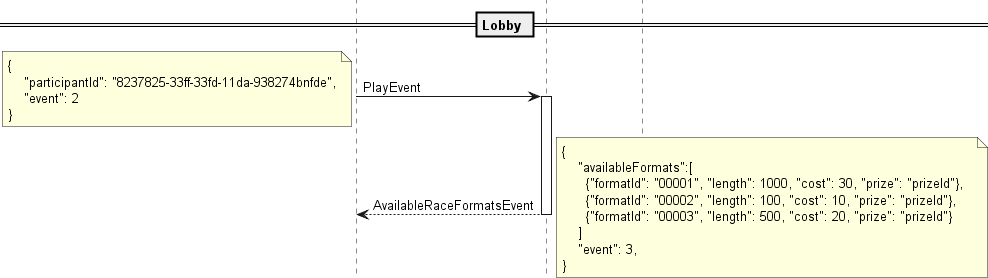
\includegraphics[width=14.5cm]{figure/RacesFormats.png}
            \caption{Diagramma di sequenza per gli eventi GetAvailableRacesEvent e OnAvailableRacesFormatsEvent}
            \label{img:PlayEvent}
        \end{figure}

        L'evento \textit{PlayEvent} viene innescato quando il giocatore preme il pulsante \textit{Start}, come visto in Algoritmo: \ref{alg:StartWidget}.
        %
        Il delegate in questione è legato alla funzione vista in Algoritmo: \ref{alg:SendMessage}.
        %
        Tramite l'esecuzione del delegate, il client invia al server il messaggio relativo all'intenzione del giocatore di voler iniziare una partita.
        %
        Il server invia in risposta un messaggio verso il client con tutte le tipologie di gare a cui è possibile accedere in quel momento.

        Il Json in arrivo dal server, come si vede nel diagramma di sequenza nella Figura: \ref{img:RacesFormats}, avrà come NumberField("event") il valore 3.
        %
        Questo valore permette di trovare nella mappa degli eventi con la funzione vista in Algoritmo:\ref{alg:OnMessageReceived} la funzione \textit{OnAvailabelRaceFormatsEvent}.

        \begin{lstlisting}[caption = Funzione OnAvailabelRaceFormatsEvent, label = {alg:OnAvailabelRaceFormatsEvent}]
void AMetaraceNetworkActor::OnAvailableRacesFormatsEvent(AMetaraceNetworkActor* NetworkActor, const FJsonObject& JsonObject)
{
    UAvailableRacesFormatsEventDTO* Dto = 
        NewObject<UAvailableRacesFormatsEventDTO>();
    Dto->AddToRoot();

    const TArray<TSharedPtr<FJsonValue>> AvailableFormatsJson = 
        JsonObject.GetArrayField("availableFormats");
    for(auto Format : AvailableFormatsJson)
    {
        URaceFormatObject* RaceFormat = 
            NewObject<URaceFormatObject>();
        RaceFormat->Id = Format.Get()->AsObject()
            .Get()->GetStringField("formatId");
        RaceFormat->Length = Format.Get()->AsObject()
            .Get()->GetStringField("length");
        RaceFormat->Cost = Format.Get()->AsObject()
            .Get()->GetStringField("cost");
        RaceFormat->Prize = Format.Get()->AsObject()
            .Get()->GetStringField("prize");
        Dto->Formats.Add(RaceFormat);		
    }

    if(NetworkActor && NetworkActor->OnAvailableRacesFormatsEventDelegate.IsBound())
    {
        NetworkActor->OnAvailableRacesFormatsEventDelegate.Execute(Dto);
    }
}
        \end{lstlisting}

        Come si vede in Algoritmo: \ref{alg:OnAvailabelRaceFormatsEvent} il file Json viene spacchettato e salvato dentro un oggetto DTO.
        %
        Il delegate relativo a questo evento viene quindi eseguito passando l'oggetto DTO appena creato.
        %
        Il delegate, come visto nella funzione \textit{Begin Play} dell'\textit{ApplicationManager} (Algoritmo: \ref{alg:bindDelegate}), è legato alla funzione \textit{ShowAvailableRacesFormats} implementata nello \textit{SceneController}.
        %
        Questa funzione a sua volta passa gli oggetti rappresentati i formati della gara al \textit{WidgetController} che si occuperà di farli visualizzare al giocatore sotto forma di bottoni per poter scegliere a quale gara partecipare.

        \subsubsection{JoinEvent e PlayerJoinedEvent}

        \begin{figure}[b]\label{img:JoinEvent}
            \centering
            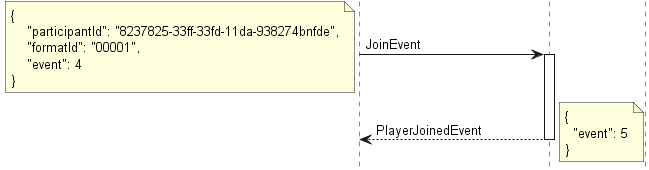
\includegraphics[width=13cm]{figure/JoinEvent.png}
            \caption{Diagramma di sequenza per gli eventi JoinEvent e PlayerJoinedEvent}
        \end{figure}

        L'evento \textit{JoinEvent} viene innescato quando un giocatore preme su un bottone corrispettivo ad una specifica tipologia di gara.
        %
        Similmente a come accade con il bottone \textit{Start} (Algoritmo: \ref{alg:StartWidget}), l'esecuzione del delegate permette di inviare al server un messaggio rappresentante la gara scelta.
        %
        Il formato del file Json in questione è descritto nella Figura: \ref{img:JoinEvent}.
        

        Il server alla ricezione del messaggio inserisce il giocatore in questione nella gara scelta e invia un messaggio di conferma avvenuta connessione alla gara: questo è l'evento \textit{PlayerJoinedEvent}.
        %
        Anche questo evento è mappato dentro lo \textit{SceneController} e permette di passare alla vista di gara.

        \subsubsection{StartingGridEvent e AnotherPlayerJoinedEvent}

        \begin{figure}[!ht]\label{img:StartingGrid}
            \centering
            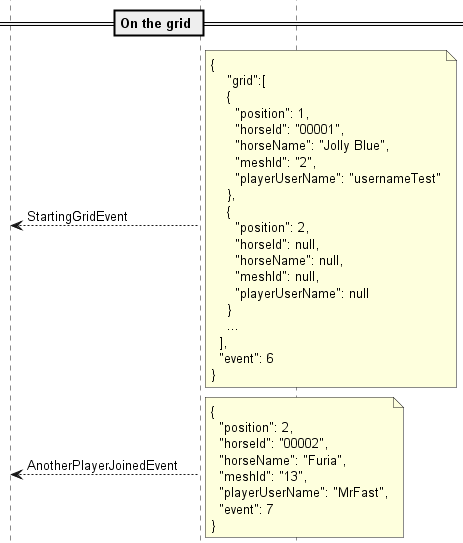
\includegraphics[width=10cm]{figure/StartingGrid.png}
            \caption{Diagramma di sequenza per gli eventi StartingGridEvent e AnotherPlayerJoinedEvent}
        \end{figure}

        Questi due eventi permettono al client di ricevere le informazioni riguardanti la gara alla quale si è connesso.
        %
        L'evento \textit{StartingGridEvent} permettere di ricevere le informazioni della griglia di partenza presente al momento della connessione alla gara, quindi arriveranno tutte le informazioni dei cavalli in attesa dell'avvio della gara già presenti sulla griglia.
        %
        Il file Json in Figura \ref{img:StartingGrid} è un esempio di griglia di partenza.
        %
        L'evento \textit{AnotherPlayerJoinedEvent} permette di ricevere le informazioni dei giocatori che si connetteranno alla gara successivamente.
        %
        Ne arriverà uno per ogni giocatore aggiuntivo che si connette.
        
        \begin{lstlisting}[caption = Funzione che spacchetta il file Json per la griglia iniziale, label = {alg:StartingGrid}]
void AMetaraceNetworkActor::OnStartingGridEvent(
    AMetaraceNetworkActor* NetworkActor, const FJsonObject& JsonObject)
{
    UStartingGridEventDTO* Dto = NewObject<UStartingGridEventDTO>();
    Dto->AddToRoot();

    const TArray<TSharedPtr<FJsonValue>> PlayersArrayJson = 
        JsonObject.GetArrayField("horses");
    
    for(TSharedPtr<FJsonValue> horse : PlayersArrayJson)
    {		
        UHorseObject* H = NewObject<UHorseObject>();
        H->Name = horse.Get()->AsObject().Get()->GetStringField("horseName");
        H->Id = horse.Get()->AsObject().Get()->GetStringField("horseId");
        H->MeshReference = horse.Get()->AsObject().Get()->GetNumberField("mesh");
        H->Position = horse.Get()->AsObject().Get()->GetNumberField("position");
        
        Dto->Players.Add(H);
    }

    if(NetworkActor && 
        NetworkActor->OnStartingGridEventDelegate.IsBound())
    {
        NetworkActor->OnStartingGridEventDelegate.Execute(Dto);
    }
}            
        \end{lstlisting}

        L'esecuzione di questo delegete chiama la funzione dello \textit{SceneController} che si occupa dello spawn dei cavalli (Algoritmo \ref{alg:SpawnHorses}):

        \begin{lstlisting}[caption = Funzione in \textit{SceneController} che fa comparire i cavalli, label={alg:SpawnHorses}]
void AMetaraceSceneController::StartingGrid(
    const UStartingGridEventDTO* StartingGridEventDto)
{
    UWorld* World = GetWorld();
    if(!World) { return; }
    
    FActorSpawnParameters SpawnParams;
    if(BP_Horse)
    {
        for(UHorseObject* HorseObject : 
            StartingGridEventDto->Players)
        {
            int32 Position = HorseObject->Position;
            FTransform SpawnTransform = 
                Splines[Position]->GetTransformAtSplinePoint(
                    0, ESplineCoordinateSpace::World);
            AHorse* Horse = World->SpawnActor<AHorse>(
                BP_Horse, SpawnTransform, SpawnParams);
            Horse->SetSkeletalMesh(
                    Int2Mesh[HorseObject->MeshReference]);
            Horse->SetSplineComponent(Splines[Position]);
            Horse->Name = HorseObject->Name;
            Horse->Id = HorseObject->Id;
                        
            //I riferimenti ai cavalli vengono tenuti in una TMap
            Horses.Add(Horse->Id, Horse);
        }
    }
}
        \end{lstlisting}

        \subsubsection{CountdownEvent e RaceEvent}

        \begin{figure}[!ht]\label{img:CountdownEvent}
            \centering
            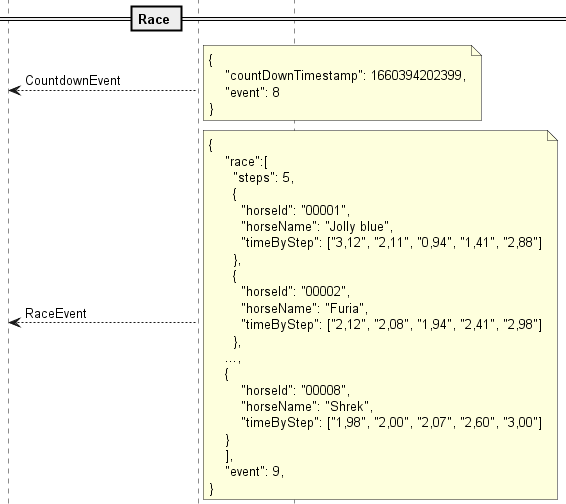
\includegraphics[width=11cm]{figure/CountdownEvent.png}
            \caption{Diagramma di sequenza per gli eventi CountdownEvent e RaceEvent}
        \end{figure}

        Il \textit{CountdownEvent} è un evento che parte dal server per sincronizzare tutti i client partecipanti alla gara.
        %
        Esso viene lanciato dal server nel momento in cui le condizioni per poter iniziare la partita sono state raggiunte.
        %
        Le condizioni sono: il raggiungimento del numero massimo dei partecipanti oppure la scadenza di un conto alla rovescia partito al raggiungimento del numero minimo dei partecipanti.
        %
        Il file Json associato a questo evento, come si vede nella Figura \ref{img:CountdownEvent}, porta con se solo la durata del timer rimanente per l'inizio della gara.
        %
        In Unreal Engine ci sono degli oggetti appositamente creati per la gestione del conto alla rovescia, i \textit{FTimerHandle}.
        %
        I timer in Unreal Engine permettono di definire una funzione da chiamare allo scadere del tempo impostato.
        %
        La funzione dello SceneController chiamata dal delegate di questo evento comunica la durata del countdown al WidgetController - che si occupa di fare il display del conto alla rovescia - e sfrutta un \textit{FTimerHandle} per far partire la gara - con la funzione \textit{StartRace} - allo scadere del tempo comunicato dal server.

        \begin{lstlisting}[caption = Funzione nello SceneController che inizializza un \textit{FTimerHandle}]
void AMetaraceSceneController::ShowCountDown(
    const UCountdownEventDTO* CountdownEventDto)
{	
	WidgetController->ShowCountdown(
            CountdownEventDto->CountdownTimestamp);
	
	FTimerHandle TimerHandle2;
	GetWorldTimerManager().SetTimer(TimerHandle2, this, 
        &AMetaraceSceneController::StartRace, 1.f, false,
        CountdownEventDto->CountdownTimestamp);
}
        \end{lstlisting}

        Il \textit{RaceEvent} è un altro evento che parte dal server e viene lanciato consecutivamente al \textit{CountdownEvent}.
        %
        Il file Json associato a questo evento porta tutte le informazioni per lo svolgersi della gara.
        %
        Questo è il file che contiene l'insieme degli array dei tempi di cui si è discusso nel Paragrafo \ref{sec:Meccanica}, ossia l'insieme dei tempi con cui il cavallo percorrerà ciascuno step del percorso.

        \begin{lstlisting}[caption = Funzione che spacchetta il file Json relativo ai dati di gara, label = {alg:OnRaceEvent}]
void AMetaraceNetworkActor::OnRaceEvent(AMetaraceNetworkActor* NetworkActor, 
    const FJsonObject& JSonObject)
{
    URaceEventDTO* Dto = NewObject<URaceEventDTO>();
    Dto->AddToRoot();

    Dto->NumStep = JSonObject.GetNumberField("step");

    const TArray<TSharedPtr<FJsonValue>> HorsesJson = 
        JSonObject.GetArrayField("horses");
    for(TSharedPtr<FJsonValue> Horse : HorsesJson)
    {
        UHorseObject* H = NewObject<UHorseObject>();
        H->Id = Horse.Get()->AsObject()
            .Get()->GetStringField("horseId");
        const TArray<TSharedPtr<FJsonValue>> TimeArrayJson = 
            Horse.Get()->AsObject().Get()->GetArrayField("timeByStep");

        for(auto Time : TimeArrayJson)
        {
            H->TimeArray.Add(Time.Get()->AsNumber());
        }
        Dto->Horses.Add(H);
    }
    
    if(NetworkActor && NetworkActor->OnRaceEventDelegate.IsBound())
    {
        NetworkActor->OnRaceEventDelegate.Execute(Dto);
    }
}
        \end{lstlisting}

        La funzione dello \textit{SceneController} chiamata dal delegate per il RaceEvent in Algoritmo \ref{alg:OnRaceEvent}, si occupa di passare l'array di tempi ai cavalli e di chiamare la funzione \textit{Inizialize} vista in Algoritmo: \ref{alg:HorseInizialize}.

        \begin{lstlisting}[caption = Funzione dello SceneController che inizializza i cavalli]
void AMetaraceSceneController::InitRace(
    const URaceEventDTO* StartRaceEventDto)
{
	for(auto HorseObject : StartRaceEventDto->Horses)
	{
		AHorse* Horse = *Horses.Find(HorseObject->Id);
		Horse->TimeArray = HorseObject->TimeArray;
		Horse->Inizialize();
	}
}
        \end{lstlisting}

        \subsubsection{RaceFinishedEvent e Leaderboardevent}

        L'evento \textit{RaceFinishedEvent} viene lanciato dallo SceneController stesso.
        %
        Infatti, in scena è presente un \textit{ATriggerBox} in corrispondenza del traguardo che al verificarsi dell'\textit{OverlapEvent} (ossia quando i cavalli raggiungono il traguardo) chiama la funzione che genera e invia il file Json relativo a questo evento.
        %
        L'obiettivo di questo evento è quella di far sapere al server che il client ha fatto visualizzare l'intera gara e che aspetta i dati per fare il display della \textit{Leaderboard}.
        %
        Questo è il motivo per cui anche lo SceneController ha un delegate legato alla funzione \textit{SendMessage} del NetworkActor, Algoritmo \ref{alg:SendMessage}.

        \begin{figure}[t]
            \centering
            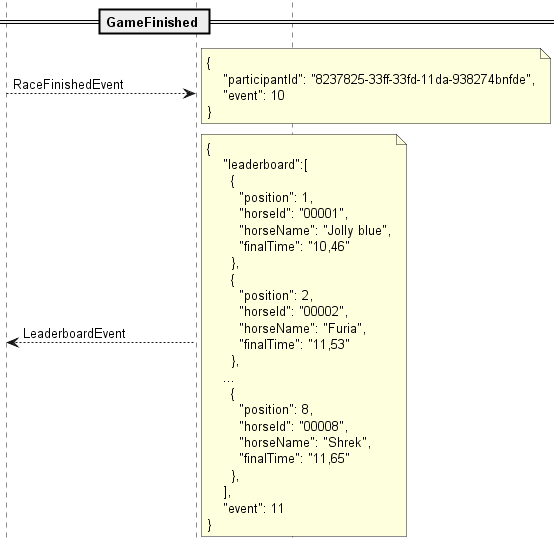
\includegraphics[width=12cm]{figure/RaceFinishedEvent.png}
            \caption{Diagramma di sequenza per gli eventi RaceFinishedEvent e LeaderboardEvent}
        \end{figure}